% !TEX root = ../../../main.tex

\toggletrue{image}
\toggletrue{imagehover}
\chapterimage{security_question}
\chapterimagetitle{\uppercase{Security Question}}
\chapterimageurl{https://xkcd.com/565/}
\chapterimagehover{Let's invite him to a party and play 'I never'. Okay, I never hid any bodies SOUTH of Main Street. ...he's taking a drink!}

\chapter{Perfekte Sicherheit}
\label{chapter-perfekte-sicherheit}

Alle bisher vorgestellten Kryptosysteme sind nicht sicher. Wir klären nun, wie wir perfekte (vollkommene) Sicherheit erreichen können. Die Lernziele lauten wie folgt:

\newcommand{\perfekteSicherheitLernziele}{
\protect\begin{todolist}
\item Sie erklären, was wir unter perfekter Sicherheit verstehen.
\item Sie nennen die Kriterien, damit ein Kryptosystem perfekt sicher ist.
\item Sie wenden alle vorgestellten, perfekt sicheren Kryptosysteme an.
\item Sie erklären, warum perfekt sichere Kryptosysteme in der Praxis kaum zum Einsatz kommen.
\end{todolist}
}

\lernziel{\autoref{chapter-perfekte-sicherheit}, \nameref{chapter-perfekte-sicherheit}}{\protect\perfekteSicherheitLernziele}

\perfekteSicherheitLernziele

\section{Wann ist ein Kryptosystem perfekt sicher?}
\label{section-kryptosystem-perfekt-sicher}

Intuitiv ist ein Kryptosystem perfekt sicher, wenn es keinem Kryptoanalytiker möglich ist (egal wie viel Zeit, Rechenkapazität und Wissen investiert wird), aus einem Kryptotext eine Kenntnis über den Klartext\footnote{Mit Ausnahme der Klartextlänge.} oder den Schlüssel zu erlangen. Im Jahr 1949 definierte Claude Shannon den Begriff etwas formaler.

\begin{definition}[Perfekte Sicherheit]
Ein Kryptosystem ist für Klartexte und Kryptotexte der \textbf{Länge $n$} perfekt sicher, wenn folgende Bedingungen erfüllt sind:

\begin{enumerate}
	\item Jeder Schlüssel besitzt die Länge $n$. 
	\item Die $n$ Schlüsselwortzeichen werden zufällig gewählt. Jedes Schlüsselwortzeichen ist gleich wahrscheinlich.
	\item Für jeden Klartext wird ein neuer Schlüssel erzeugt.
	\item Die Anzahl der möglichen Klartexte ist identisch mit der Anzahl der möglichen Schlüssel und der Anzahl der möglichen Kryptotexte.
\end{enumerate}

\end{definition}

In einem perfekt sicheren Kryptosystem lässt der Kryptotext \textbf{keinerlei Rückschlüsse} auf den Klartext zu. Für jeden \textbf{Klartext} und den dazugehörigen \textbf{Kryptotext} gibt es somit \textbf{exakt einen Schlüssel}. Daraus folgt, dass ein Klartext unabhängig	vom Kryptotext ist, wenn wir den Schlüssel nicht besitzen. Die Anforderungen an ein perfektes Kryptosystem sind hoch. Es schränkt die Gestaltung von Kryptosystem stark ein. Wir zeigen nun jedoch Kryptosysteme, welche bei korrekter Anwendung, perfekte Sicherheit bieten.

\section{Das Kryptosystem \texttt{VIGENÈRE-PLUS}}

Wir verbessern das Kryptosystem \texttt{VIGENÈRE}, um ein perfekt sicheres Kryptosystem zu erhalten. Wir nennen dieses Kryptosystem \texttt{VIGENÈRE-PLUS}.

\subsection{Verschlüsselung und Entschlüsselung}

Die \textbf{Verschlüsselung} erfolgt analog zu \texttt{VIGENÈRE}. Pro Klartextbuchstabe führen wir diese Schritte durch:

\begin{enumerate}
	\item Bestimmte die Klartextlänge $n$.
	\item Erzeuge einen Schlüssel der Länge $n$. Jeder Schlüsselwortbuchstabe muss zufällig gewählt werden. Jeder Schlüsselwortbuchstabe ist gleich wahrscheinlich.
	\item Der Klartext wird mit dem Schlüssel gemäss \texttt{VIGENÈRE} verschlüsselt.
\end{enumerate}

Für jeden Klartext müssen wir einen \textbf{neuen Schlüssel} benutzen. Wir können zum Beispiel die Website \url{www.random.org/strings} benutzen, um einen zufälligen Schlüssel zu erzeugen.

\begin{example}
	Wir verschlüsseln PARTY mit MRQUO und erhalten BRHNM.
\end{example}

Die \textbf{Entschlüsselung} ist identisch zu \texttt{VIGENÈRE}.

\begin{example}
	Wir entschlüsseln RPHYR mit QHQLN und erhalten BIRNE .
\end{example}

\subsection{Aufgaben}

Bei allen Aufgaben ist das Kryptosystem \texttt{VIGENÈRE-PLUS} zu verwenden.

\begin{enumerate}

\item Der Kryptotext lautet TLSPAWPCKWQECWKF. Es wurde der Schlüssel TTZLJOSIXTCDYLCI benutzt. Wie lautet der Klartext?

\fillwithgrid{1in}

\item Verschlüsseln Sie den Klartext UEBERRASCHUNGSEI. Erzeugen Sie mit der Website \url{www.random.org/strings} einen passenden Schlüssel.

\fillwithgrid{1in}

\item Wie viele \textbf{verschiedene Schlüssel} gibt es, wenn der Klartext eine Länge von $n$ besitzt und \num{26} Buchstaben benutzt werden. Geben Sie eine \textbf{allgemeine Formel} an und \textbf{berechnen} Sie die Anzahl für $n = 10$.

\fillwithgrid{\stretch{1}}

\end{enumerate}

\newpage

\section{Das Kryptosystem \texttt{ONE-TIME-PAD}}

Das Kryptosystem wurde 1917 von Gilbert S. Vernam zum Patent angemeldet. Claude Shannon bewies in den 1940er-Jahren, dass das Kryptosystem perfekt sicher ist. Das Kryptosystem \texttt{ONE-TIME-PAD} funktioniert analog zum Kryptosystem \texttt{VIGENÈRE-PLUS}. Der Unterschied besteht darin, dass beim Kryptosystem \texttt{ONE-TIME-PAD} Binärzahlen benutzt werden.

\subsection{Verschlüsselung und Entschlüsselung}

Die \textbf{Verschlüsselung} erfolgt durch eine Codierung der Zeichen. Wir führen dazu folgende Schritte durch:

\begin{enumerate}
	\item \label{item-cipher-one-time-pad-1} \textbf{Codiere} den \textbf{Klartext} mit einem \textbf{Binärcode} (z.B. \ac{ASCII}).
	\item Bestimme die \textbf{Länge} $n$ des \textbf{codierten} Klartextes.
	\item \label{item-cipher-one-time-pad-2} Erzeuge einen Schlüssel der Länge $n$. \textbf{Der Schlüssel besteht aus $n$ Bits}. Wähle jedes Bit \textbf{zufällig} mit gleicher Wahrscheinlichkeit aus.
	
	\item \label{item-cipher-one-time-pad-3} \textbf{Addiere} die beiden Binärzahlen aus \ref{item-cipher-one-time-pad-1}. und \ref{item-cipher-one-time-pad-2}. \textbf{bitweise} mit $\bmod 2$.
	\item Das Ergebnis aus \ref{item-cipher-one-time-pad-3}. sind $n$ Bits. Diese $n$ Bits stellen den \textbf{Kryptotext} dar.
\end{enumerate}

Wir können einen Schlüssel zum Beispiel mit der Website \url{www.random.org/bytes} erzeugen.

\begin{important}
Die bitweise, modulare Addition bedeutet, dass \textbf{Bit für Bit} separat $\bmod 2$ addiert wird. Es gibt keinen Übertrag.
\end{important}

\begin{example}
Das Kryptosystem \texttt{ONE-TIME-PAD} erlaubt nun auf einfache Weise einen Klartext mit beliebigen Zeichen zu verschlüsseln. Wir verschlüsseln deshalb nun den Klartext 15 UHR.

% 15 UHR => ASCII
% 0110001 0110101 0100000 1010101 1001000 1010010
% KSWE => ASCII
% 1001011 1010011 1010111 1000101

\begin{table}[htb]
\centering
\resizebox{\textwidth}{!}{%
\begin{tblr}{
    colspec = {|Q[c, m]|Q[c, m]|Q[c, m]|Q[c, m]|Q[c, m]|Q[c, m]|Q[c, m]|Q[c, m]|Q[c, m]|Q[c, m]|Q[c, m]|Q[c, m]|Q[c, m]|Q[c, m]|}
}
\hline
Klartext   		& 1 & 5 & $\sqcup$ & U & H & R & $\xrightarrow[\acs{ASCII}]{\makebox[2cm]{Codieren}}$ 
			& 0110001 & 0110101 & 0100000 & 1010101 & 1001000 & 1010010 \\ \hline
  			& & & & & & & Schlüssel 
			& 0001111 & 1010000 & 1011110 & 1000100 & 0001111 & 0111101 \\ \hline
  			&  &  &  &  &  & & bitweise $\oplus_2$ 
			& 0111110 & 1100101 & 1111110 & 0010001 & 1000111 & 1101111 \\ \hline
\end{tblr}
}
\end{table}

Der \textbf{Kryptotext} besteht aus den Bits, welche nach der bitweisen, modularen Addition entstehen. In diesem Beispiel also $110001011000101100101001111000110110000001$. Wir zeigen hier noch detailliert, wie die Berechnung der ersten \num{7} Bits des Kryptotextes durchgeführt werden.

\begin{table}[htb]
\centering
\resizebox{\textwidth}{!}{%
\begin{tblr}{
    colspec = {|Q[c, m]|Q[c, m]|Q[c, m]|Q[c, m]|Q[c, m]|Q[c, m]|Q[c, m]|Q[c, m]|}
}
\hline
Klartext      	& 0 & 1 & 1 & 0 & 0 & 0 & 1 \\ \hline
Schlüssel     	& 0 & 0 & 0 & 1 & 1 & 1 & 1 \\ \hline
{bitweise, \\ modulare \\ Addition} & 
$0 \oplus_2 0 = 0$ & 
$1 \oplus_2 0 = 1$ & 
$1 \oplus_2 0 = 1$ & 
$0 \oplus_2 1 = 1$ & 
$0 \oplus_2 1 = 1$ & 
$0 \oplus_2 1 = 1$ & 
$1 \oplus_2 1 = 0$ \\ \hline[2pt]
Kryptotext    & 0 & 1 & 1 & 1 & 1 & 1 & 0 \\ \hline
\end{tblr}
}
\end{table}

\end{example}

Das Praktische beim Kryptosystem \texttt{ONE-TIME-PAD} ist die Einfachheit. Das \textbf{Entschlüsseln} eines Kryptotextes funktioniert \textbf{identisch} zum \textbf{Verschlüsseln}. Dies liegt daran, dass bei $\oplus_2$ und $\mathbb{Z}_2$ die modulare Addition zweier Bits identisch ist mit der modularen Subtraktion zweier Bits. Die Schritte lauten deshalb wie folgt:

\begin{enumerate}
	\item Notiere den Schlüssel unterhalb des Kryptotextes. 
	\item \label{item-decipher-one-time-pad-2} Führe die bitweise, modulare Addition mit $\bmod 2$ durch.
	\item Wir erhalten den Klartext, in dem wir das Ergebnis aus \ref{item-decipher-one-time-pad-2}. decodieren.
\end{enumerate}
	
\begin{example}
	Wir entschlüsseln den Kryptotext 01010001101001100000011110111100110 und verwenden den Schlüssel 11010111000100111001101010110101001.

% C-3PO 		1000011	0101101	0110011	1010000	1001111
% Schlüssel	1101011	1000100	1110011	0101011	0101001
% Kryptotext	0101000	1101001	1000000	1111011	1100110

\begin{table}[htb]
\centering
\resizebox{\textwidth}{!}{%
\begin{tblr}{
    colspec = {|Q[c, m]|Q[c, m]|Q[c, m]|Q[c, m]|Q[c, m]|Q[c, m]|Q[c, m]|Q[c, m]|}
}
\hline
& & & & & & Kryptotext & \texttt{01010001101001100000011110111100110} \\ \hline
& & & & & & Schlüssel & \texttt{11010111000100111001101010110101001} \\ \hline
& & & & & & bitweise $\oplus_2$ & \texttt{10000110101101011001110100001001111} \\ \hline
Klartext & C & - & 3 & P & 0 & $\xleftarrow[\acs{ASCII}]{\makebox[2cm]{Decodieren}}$ &  \texttt{1000011 0101101 0110011 1010000 1001111} \\ \hline
\end{tblr}
}
\end{table}
\end{example}

\subsection{\texttt{XOR} und $\bmod 2$}

In der Praxis (z.B. beim Programmieren oder bei Hardwarekomponenten) greifen wir bei der Umsetzung des Kryptosystems \texttt{ONE-TIME-PAD} auf den \textbf{\texttt{XOR}-Operator} bzw. das \textbf{\texttt{XOR}-Gate} zurück, da dies \textbf{einfacher} und \textbf{schneller} ist. Dies ist möglich, weil $\bmod 2$ gerade dem \texttt{XOR}-Operator bzw. \texttt{XOR}-Gate entspricht (siehe \autoref{figure-xor-mod2}). 

\begin{figure}[htb]
	\centering
	\begin{minipage}{0.45\textwidth}
		\centering
		\begin{tblr}{
    			colspec = {|c|c|[2pt]c|}
		}
		\hline
		A & B & $A \oplus_2 B$ \\ \hline[2pt]
		0 & 0 & 0     \\ \hline
		0 & 1 & 1     \\ \hline
		1 & 0 & 1     \\ \hline
		1 & 1 & 0     \\ \hline
		\end{tblr}
	\end{minipage}
	\begin{minipage}{0.45\textwidth}
		\centering
		\begin{tblr}{
    			colspec = {|c|c|[2pt]c|}
		}
		\hline
		A & B & A \texttt{XOR} B \\ \hline[2pt]
		0 & 0 & 0     \\ \hline
		0 & 1 & 1     \\ \hline
		1 & 0 & 1     \\ \hline
		1 & 1 & 0     \\ \hline
		\end{tblr}
	\end{minipage}
	\caption{$\oplus_2$ und \texttt{XOR} erzeugen bei zwei Binärziffern die identischen Resultate.}
	\label{figure-xor-mod2}
\end{figure}

\begin{lstlisting}[language=python, mathescape=true, caption={In Python können wir mit $~\hat{}~$ den \protect\say{bitwise exclusive or}-Operator einsetzen. Mit \protect\lstinline{0b} kennzeichnen wir in Python eine Binärzahl.}, label={lst-python-xor}]
a = 0b00101
b = 0b10110
c = a $\hat{}$ b
\end{lstlisting}

Die Verschlüsselung und Entschlüsselung können wir somit auch mit dem bitweisen \texttt{XOR}-Operator durchführen. Bei der \say{manuellen} Durchführung ist noch folgende Beobachtung von Vorteil:

\begin{important}
	Sowohl bei der modularen Addition mit $\bmod 2$ als auch mit dem bitweisen \texttt{XOR}-Operator ist das Ergebnis nur dann 0, falls zwei identische Binärziffern (0 und 0 bzw. 1 und 1) addiert bzw. verknüpft werden. Sonst ist das Ergebnis 1.
\end{important}

\newpage

\subsection{Aufgaben}

Bei allen Aufgaben ist das Kryptosystem \texttt{ONE-TIME-PAD} zu verwenden. Sie finden im Anhang eine \ac{ASCII}-Tabelle.

\begin{enumerate}

\item \textbf{Kryptotext} (a) und \textbf{Schlüssel} (b) sind gegeben. Wie lautet der \textbf{Klartext}?\\ 
(a) \texttt{101110001101010011000011111001101101001100000100011001111110010}\\ 
(b) \texttt{000111111000011011001110110000101100011011100100101101010100001}

% STAR WARS
% 1010011 1010100 1000001 1010010 0100000 1010111 1000001 1010010 1010011
% Schlüssel
% 000111111000011011001110110000101100011011100100101101010100001
% Kryptotext
% 101110001101010011000011111001101101001100000100011001111110010

\fillwithgrid{1in}

\item Verschlüsseln Sie den Klartext BB-8. Erzeugen Sie mit \url{www.random.org/bytes} einen passenden Schlüssel. Sie müssen auf der Website die \textbf{passende Anzahl Bytes} auswählen und unter \say{How do you want your bytes displayed?} die Option \textbf{\say{Binary}} anwählen.

\fillwithgrid{1.5in}

\item Wie viele \textbf{verschiedene Schlüssel} gibt es, wenn der Klartext eine \textbf{Länge von $n$ \ac{ASCII}-Zeichen} besitzt. Geben Sie eine\textbf{ allgemeine Formel} an und \textbf{berechnen} Sie die Anzahl für $n = 10$.

\fillwithgrid{2in}

\item \textbf{Klartext} (a) und \textbf{Kryptotext} (b) sind gegeben. Wie lautet der \textbf{Schlüssel}?\\
(a) \texttt{01001011010011000100111101010011010101000100010101010010} \\
(b) \texttt{00001010010111101001110111101101001000111001011100110011}

% Kloster
% 01001011010011000100111101010011010101000100010101010010
% Schlüssel
% 1000001000100101101001010111110011101111101001001100001

\fillwithgrid{1in}

\newpage

\item Alice verwendet One-Time-Pad. Sie stellt fest, wenn der Schlüssel aus lauter Nullen besteht, dann wird ihre Nachricht quasi unverschlüsselt gesendet.
\begin{enumerate}
\item Zeigen Sie an einem Beispiel, dass Alice recht hat.
\fillwithgrid{2in}
\item Wie lautet die Wahrscheinlichkeit einen Schlüssel ausschliesslich bestehend aus $n$ Nullen zu erzeugen?
\fillwithgrid{2in}
\item Bob schlägt vor, bei der Schlüsselerzeugung den Schlüssel mit lauter Nullen zu verbieten. Er nennt das Kryptosystem \texttt{ONE-TIME-PAD-PLUS}. Ist dieses Kryptosystem perfekt sicher? Begründen Sie Ihre Antwort hinsichtlich der vier Kriterien aus \autoref{section-kryptosystem-perfekt-sicher}.
\fillwithgrid{2in}
\end{enumerate}
\end{enumerate}

\newpage

\section{Kryptoanalyse: Wenn wir einen Schlüssel mehrfach benutzen}

Das Kryptosystem \texttt{ONE-TIME-PAD} schränkt die Wahl des Schlüssels ein. Wir möchten nun darauf eingehen, was passiert wenn wir eine Bedingung an den Schlüssel nicht einhalten. Wir greifen hier folgende Bedingung auf:

\begin{center}
	Für jeden Klartext wird ein neuer Schlüssel erzeugt.
\end{center}

Wie kann Eve den Kryptotext knacken, falls wir denselben Schlüssel zwei Mal benutzen? Wir zeigen dies mit einem Kryptotext der Länge \num{5}. \autoref{figure-one-time-pad-crack-1} zeigt die Ausgangssituation von Eve.

\begin{figure}[htb]
\centering
\begin{tikzpicture}
\node [cloud, draw, cloud puffs=7, cloud puff arc=120, aspect=3, text width=2.5cm, align=center] (medium) at (0,0) {\footnotesize Übertragungsmedium};

\node[inner sep=0pt] (alice) at (-6,2)
    {
\includegraphics[scale=0.25]{alice_tiny}};
\node[text width=2cm, align=center] (sender) at (-5, 2) {Sender (Alice)};
\node[rectangle, fill=black!25] (ver) at (-5.5, 0) {Verschlüsselung};
\draw[-latex, very thick] (alice.south west) -- (ver.north) node[left, midway] {Klartext};
\draw[-latex, very thick] (sender.south) -- (ver.north) node[right, midway] {Schlüssel};
\draw[-latex, very thick] (ver.east) -- (medium.west) node[above, midway] {Kryptotext} node[below, midway] {GVRCL};

\node[inner sep=0pt] (bob) at (5,2)
    {
\includegraphics[scale=0.25]{bob_tiny}};
\node[text width=2cm, align=left] (empfaenger) at (6.5, 2) {Empfänger (Bob)};
\node[rectangle, fill=black!25] (entsch) at (5.5, 0) {Entschlüsselung};
\draw[-latex, very thick] (entsch.north) -- (5.5, 1.5) node[right, midway] {Klartext};
\draw[-latex, very thick] (5, 1.5) -- (5, 0.25) node[left, midway] {Schlüssel};
\draw[-latex, very thick] (medium.east) -- (entsch.west) node[above, midway] {Kryptotext} node[below, midway] {GVRCL};

\node[inner sep=0pt] (eve) at (-0.75,-3)
    {
\includegraphics[scale=0.25]{eve_tiny}};
\node[text width=3cm, align=center] (pangreifer) at (0.75, -3) {Passiver Angreifer (Eve)};
\draw[-latex, very thick] (medium.south) -- (0, -2.5) node[right, midway] {Kryptotext (Kopie): GVRCL};

\end{tikzpicture}
\caption{Eve kennt nur den Kryptotext.}
\label{figure-one-time-pad-crack-1}
\end{figure}

Wir gehen davon aus, dass Alice einen Klartext in deutscher Sprache mit der Länge \num{5} an Bob schickt. Der Schlüssel besteht aus \num{5} zufälligen Buchstaben (A-Z). Eve kann \textbf{keine Häufigkeitsanalyse} durchführen. Ihr bleibt nichts anderes übrig als die \textbf{Brute-Force-Methode}. Sie muss also alle $26^5 = 11\,881\,376$ Schlüssel ausprobieren. Sie muss also für \textbf{jeden Schlüssel} den \textbf{Kryptotext} GVRCL \textbf{entschlüsseln} und \textbf{prüfen}, ob es sich um ein \textbf{sinnvolles, deutsches Wort} handelt.\\
Ein Python-Programm kann dies in circa \num{10} Minuten durchführen und dabei \textbf{mindestens 4 220 sinnvolle Wörter} für den Kryptotext GVRCL finden. Eve hat keine Chance daraus den richtigen Klartext zu ermitteln, da jedes der Wörter (theoretisch) möglich ist. \\

Da Alice nicht aufpasst, schickt sie mit demselben Schlüssel eine weitere Nachricht an Bob. Eve erhält somit einen weiteren Kryptotext, wie in \autoref{figure-one-time-pad-crack-2} dargestellt.

\begin{figure}[htb]
\centering
\begin{tikzpicture}
\node [cloud, draw, cloud puffs=7, cloud puff arc=120, aspect=3, text width=2.5cm, align=center] (medium) at (0,0) {\footnotesize Übertragungsmedium};

\node[inner sep=0pt] (alice) at (-6,2)
    {
\includegraphics[scale=0.25]{alice_tiny}};
\node[text width=2cm, align=center] (sender) at (-5, 2) {Sender (Alice)};
\node[rectangle, fill=black!25] (ver) at (-5.5, 0) {Verschlüsselung};
\draw[-latex, very thick] (alice.south west) -- (ver.north) node[left, midway] {Klartext};
\draw[-latex, very thick] (sender.south) -- (ver.north) node[right, midway] {Schlüssel};
\draw[-latex, very thick] (ver.east) -- (medium.west) node[above, midway] {Kryptotext} node[below, midway] {ADRCM};

\node[inner sep=0pt] (bob) at (5,2)
    {
\includegraphics[scale=0.25]{bob_tiny}};
\node[text width=2cm, align=left] (empfaenger) at (6.5, 2) {Empfänger (Bob)};
\node[rectangle, fill=black!25] (entsch) at (5.5, 0) {Entschlüsselung};
\draw[-latex, very thick] (entsch.north) -- (5.5, 1.5) node[right, midway] {Klartext};
\draw[-latex, very thick] (5, 1.5) -- (5, 0.25) node[left, midway] {Schlüssel};
\draw[-latex, very thick] (medium.east) -- (entsch.west) node[above, midway] {Kryptotext} node[below, midway] {ADRCM};

\node[inner sep=0pt] (eve) at (-0.75,-3)
    {
\includegraphics[scale=0.25]{eve_tiny}};
\node[text width=3cm, align=center] (pangreifer) at (0.75, -3) {Passiver Angreifer (Eve)};
\draw[-latex, very thick] (medium.south) -- (0, -2.5) node[right, midway, text width=6cm] {1. Kryptotext (Kopie): GVRCL \\2. Kryptotext (Kopie): ADRCM};

\end{tikzpicture}
\caption{Eve vermutet, dass Alice und Bob den gleichen Schlüssel verwenden.}
\label{figure-one-time-pad-crack-2}
\end{figure}

Eve weiss nun, dass beide Kryptotexte ein sinnvolles, deutsches Wort darstellen sollten. Sie führt nun erneut die \textbf{Brute-Force-Methode} durch und modifiziert dafür das Python-Programm etwas. Für jeden möglichen Schlüssel sollen nun \textbf{beide Kryptotexte} ein \textbf{sinnvolles, deutsches Wort} ergeben. Nur dann kommt der Schlüssel, welche Alice und Bob benutzt haben könnten, infrage. \autoref{lst-brute-force-one-time-pad-5-resultat} zeigt die gefundenen Klartexte und Schlüssel.

\begin{lstlisting}[language=output, label={lst-brute-force-one-time-pad-5-resultat}, caption={Es wurden \num{10} mögliche sinnvolle Klartexte für die beiden Kryptotexte gefunden.}]
Kryptotext: GVRCL, Klartext: BAREM, Schlüssel: FVAYZ
Kryptotext: ADRCM, Klartext: VIREN, Schlüssel: FVAYZ
=====================================================
Kryptotext: GVRCL, Klartext: BADEN, Schlüssel: FVOYY
Kryptotext: ADRCM, Klartext: VIDEO, Schlüssel: FVOYY
=====================================================
Kryptotext: GVRCL, Klartext: BASIS, Schlüssel: FVZUT
Kryptotext: ADRCM, Klartext: VISIT, Schlüssel: FVZUT
=====================================================
Kryptotext: GVRCL, Klartext: MALES, Schlüssel: UVGYT
Kryptotext: ADRCM, Klartext: GILET, Schlüssel: UVGYT
=====================================================
Kryptotext: GVRCL, Klartext: LACHS, Schlüssel: VVPVT
Kryptotext: ADRCM, Klartext: FICHT, Schlüssel: VVPVT
=====================================================
Kryptotext: GVRCL, Klartext: LAXES, Schlüssel: VVUYT
Kryptotext: ADRCM, Klartext: FIXET, Schlüssel: VVUYT
=====================================================
Kryptotext: GVRCL, Klartext: LAXER, Schlüssel: VVUYU
Kryptotext: ADRCM, Klartext: FIXES, Schlüssel: VVUYU
=====================================================
Kryptotext: GVRCL, Klartext: LAXEM, Schlüssel: VVUYZ
Kryptotext: ADRCM, Klartext: FIXEN, Schlüssel: VVUYZ
=====================================================
Kryptotext: GVRCL, Klartext: KALIF, Schlüssel: WVGUG
Kryptotext: ADRCM, Klartext: EILIG, Schlüssel: WVGUG
=====================================================
Kryptotext: GVRCL, Klartext: KADER, Schlüssel: WVOYU
Kryptotext: ADRCM, Klartext: EIDES, Schlüssel: WVOYU
=====================================================
\end{lstlisting}

Die Anzahl der möglichen Schlüssel, damit für \textbf{beide Kryptotexte} ein sinnvoller, deutscher Klartext entsteht, hat sich signifikant reduziert. Einer der \num{10} Schlüssel haben Alice und Bob benutzt. Welchen soll Eve wählen? Was glauben Sie?\footnote{Spoiler! Alice und Bob haben FVOYY als Schlüssel benutzt.}

\begin{important}
	Hätten Alice und Bob bei der zweiten Nachrichtenübermittlung einen neuen Schlüssel benutzt, dann hätte der Angriff von Eve nichts bewirkt.
\end{important}

\newpage

\subsection{Aufgaben}

\begin{enumerate}
	\item Alice benutzt \texttt{VIGENÈRE-PLUS}, um Bob einen Namen für die Party zu übermitteln. Es ist der geheime Ehrengast. Der Name besitzt $5$ Buchstaben.
	\begin{enumerate}
		\item Eve erhält den Kryptotext YJSLP. Sie hat Alice und Bob in letzter Zeit belauscht und vermutet, es ist ein Gast der Party. Sie glaubt, es ist ein Name mit \num{5} Buchstaben. Sie kennt den Freundeskreis von Alice und Bob und notiert sich die Namen:
			\begin{multicols}{5}
				\begin{itemize}
					\item BEATA
					\item DAVID
					\item ERWIN
					\item HANNA
					\item HELEN
					\item JAKOB
					\item JAMES
					\item JASON
					\item JONAS
					\item JULIA
					\item LAURA
					\item LINDA
					\item LUCIA
					\item LUKAS
					\item MARCO
					\item MARIA
					\item OSCAR
					\item SARAH
					\item SIMON
					\item WILMA 
				\end{itemize}
			\end{multicols}
			Erklären Sie, warum Eve den Namen nicht herausfinden kann.
			
			% ERWIN
			
			\fillwithgrid{1.5in}
			
		\item Alice schickt weitere Kryptotexte: QAHPC, BSJQC und IKYDT. Eve vermutet, dass Alice keinen neuen Schlüssel benutzt hat. Eve kann nun den gemeinsamen, geheimen Schlüssel ermitteln. Wie lauten die Klartexte? Wie lautet der Schlüssel?
		
		% WILMA, HANNA, OSCA
		
		\fillwithgrid{2.5in}
		
	\end{enumerate}
	
	\item Bei der oberen Aufgabe handelt es sich um einen Angriff mit \textbf{bekanntem Klartext}. Warum?
	
	\fillwithgrid{0.75in}
	
	\item Wie können wir in der Praxis einen Angriff mit bekanntem Klartext durchführen, wenn wir nur die Sprache des Klartextes kennen, aber keinen tatsächlichen Klartext besitzen?

	\fillwithgrid{\stretch{1}}
	
\end{enumerate}

\newpage

\section{Perfekt sichere Kryptosysteme in der Praxis: Damals und Heute}

Das One-Time-Pad hat seinen Namen daher, dass in früheren Zeiten die Schlüsselwörter auf Papier in einem Abreissblock geschrieben wurden. Diese Papierblätter wurden Pads genannt. Nach der Verwendung eines Schlüsselwortes wurde das Blatt abgerissen und vernichtet (siehe \autoref{figure-pad} für ein Beispiel).

\begin{figure}[htb]
	\centering
	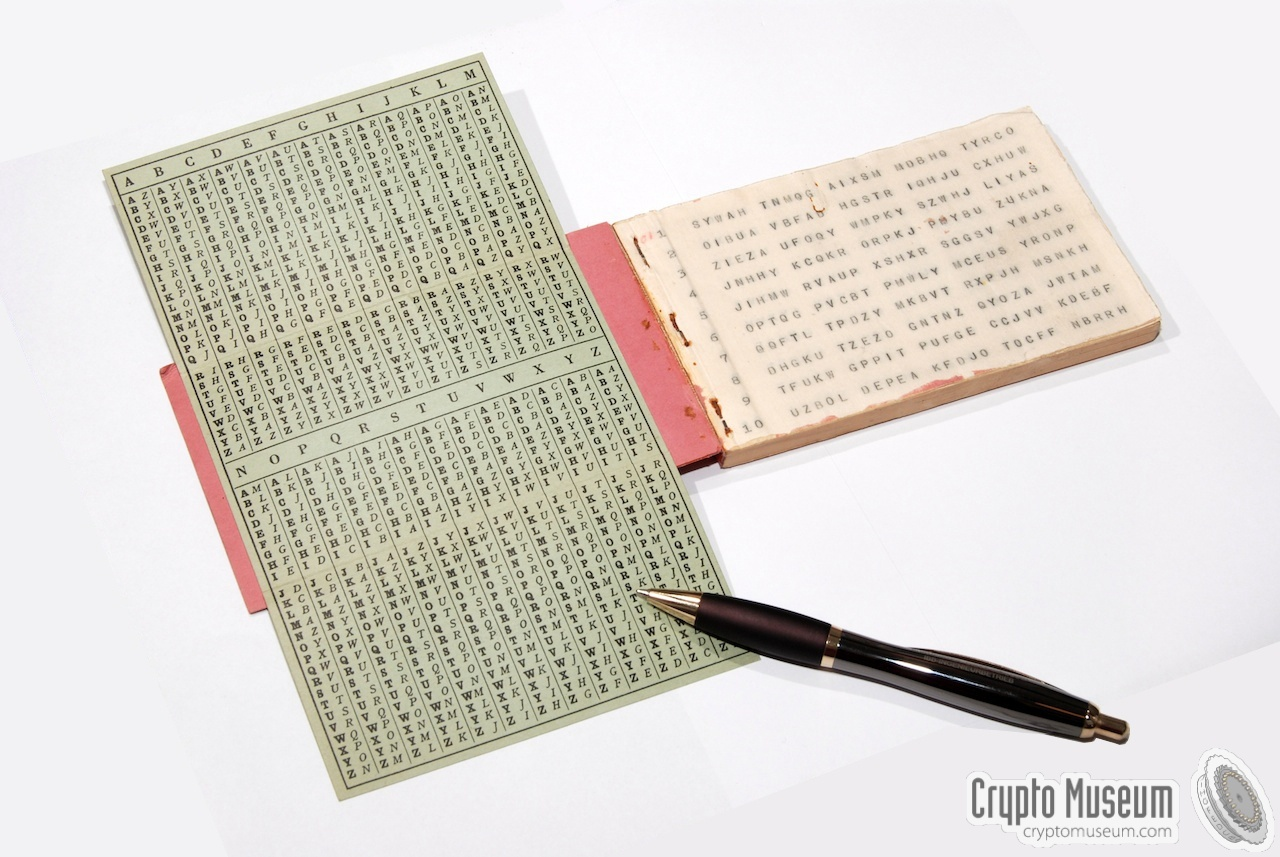
\includegraphics[width=\textwidth]{otp_abreissblock}
	\caption{Ein buchstabenbasiertes One-Time-Pad. Zirka 30 Seiten sind zusammengeheftet. Die Informationen auf dem grünen Papier wurden zur Unterstützung bei der Verschlüsselung bzw. Entschlüsselung benutzt \cite{cryptomuseum2022onetimepad}.}
	\label{figure-pad}
\end{figure}

Für den Gewinn der perfekten Sicherheit müssen wir einen hohen Aufwand betreiben. Für das \say{manuelle} \texttt{ONE-TIME-PAD} müssen wir die Schlüsselwörter auf Papier verteilen und absolut sicher aufbewahren. Deshalb wird diese Variante nur selten benutzt. Im zweiten Weltkrieg kam das Verfahren zur Übermittlung von Nachrichten aus Bletchley Park zum Premierminister zum Einsatz. In Bletchley Park war ein Team damit beschäftigt, die Enigma zu knacken. Gerüchten zufolge wurde während dem \say{Kalten Krieg} eine mit \texttt{ONE-TIME-PAD} gesicherte Gesprächsleitung zwischen dem Weissen Haus und dem Kreml eingerichtet. Ob ein aktives Gespräch jemals geführt wurde, ist unklar. Das Kryptosystem \texttt{ONE-TIME-PAD} wird kaum tatsächlich in der Praxis eingesetzt. Sender und Empfänger müssen für jeden Klartext einen Schlüssel abmachen. Und darin liegt das Problem. Entweder treffen wir uns gleich persönlich und tauschen eine grössere Anzahl von Schlüsseln aus oder wir übermitteln den Schlüssel über den gleichen Kanal wie den Kryptotext, jedoch sind die Schlüssel dann kryptografisch nicht gesichert. Sender und Empfänger können den Zeitpunkt der Übermittlung jedoch frei wählen. Dies kann jedoch dazu führen, dass die Schlüssel abgehört werden. Moderne, symmetrische Kryptosysteme verzichten deshalb auf perfekte Sicherheit. Es wird jedoch versucht, das Kryptosystem so zu entwerfen, dass der Aufwand für das Knacken in der Praxis gleichermassen unmöglich ist.

\newpage

\section{Perfekte Sicherheit $=$ Unknackbar?}

Oft hören wir im Zusammenhang mit perfekter Sicherheit folgenden Einwand: \textbf{Es gibt zwar sehr viele Schlüssel, aber wenn ich Glück habe, dann kann ich den Schlüssel doch erraten}.

Dazu geben wir die Antwort aus dem Buch \say{Kryptologie} von Albrecht Beutelspacher wieder \cite{beutelspacher2015kryptologie}:

\begin{fancyquotes}
Der Einwand ist in einem theoretischen Sinn korrekt. Zum Beispiel ist die Wahrscheinlichkeit, einen $64$-Bit-Schlüssel richtig zu raten, gleich $\frac{1}{2^{64}}$, eine Zahl, die -- darüber kann kein Zweifel bestehen -- grösser als Null ist. Um ein Gefühl dafür zu entwickeln, um \textbf{wie viel} (genauer gesagt: \textbf{um wie wenig}) diese Zahl grösser als Null ist, vergleichen wir sie mit anderen Grössen. Zunächst rechen wir die Anzahl der Schlüssel bei $64$ Bit in eine Zehnerpotenz um; es gilt $2^{64} \approx 1,94 \cdot 10^{19}$. Mit anderen Worten: Den Schlüssel zu raten, ist gleichwertig dazu, aus einer Menge von mehr als $10^{19}$ Elementen (das sind 10 Trillionen) ein spezielles Element auf Anhieb zu treffen. Können Sie sich diese Zahl vorstellen? Vielleicht helfen Ihnen die folgenden Vergleiche.

\begin{itemize}
	\item Die Weltbevölkerung beträgt derzeit etwa 8 Milliarden, also $8 \cdot 10^9$ Menschen.
	\item In einem Tropfen, also etwa einem Kubikmillimeter Wasser gibt es etwa $10^{19}$ Moleküle. Also ist das Raten des Schlüssels etwa genau so schwierig wie auf Anhieb aus einem Tropfen Wasser ein spezielles Molekül zu fischen.
	\item Erhöht man die Schlüssel auf $256$ Bit (was in der Praxis zum Beispiel bei \ac{HTTPS} möglich ist), dann erhält man $2^{256} \approx 1,15 \cdot 10^{77}$ verschiedene Schlüssel. Astronomen haben herausgefunden, dass das Universum \say{nur} ca. $10^{77}$ Elementarteilchen enthält.
	\item Die Anzahl der Möglichkeiten, beim \say{$6$ aus $49$}-Lotto einen Volltreffer zu erzielen, ist $13\,983\,816 \approx 10^7$. Das ist nämlich die Anzahl der Möglichkeiten, $6$ Zahlen aus einer Menge von $49$ Zahlen auszuwählen. Das bedeutet: Die Chance, einen $64$-Bit-Schlüssel zu raten, ist genau so gut, wie im Lotto $6$ Richtige zu haben -- und zwar in dieser Woche, in der kommenden Woche und in der übernächsten Woche!
\end{itemize}

\textbf{Moral:} Wenn Sie durch das Raten eines kryptografischen Schlüssels einen Gewinn von nur ein paar Millionen Euro erwarten, dann ist es sinnvoller, Ihr Geld beim Lotto zu verpulvern!

\end{fancyquotes}

\newpage

\section{Aufgaben}

\begin{enumerate}
	\item Gibt es eine Klartextlänge, für die \texttt{CAESAR} ein perfekt sicheres Kryptosystem ist? Begründen Sie Ihre Antwort hinsichtlich der vier Kriterien aus \autoref{section-kryptosystem-perfekt-sicher}.
	
	\fillwithgrid{2in}
	
	\item Bob behauptet, dass \texttt{CAESAR-PLUS} ein perfekt sicheres Kryptosystem ist. Prüfen Sie die vier Kriterien aus  \autoref{section-kryptosystem-perfekt-sicher} hinsichtlich \texttt{CAESAR-PLUS}. Welches Kriterium können wir mit \texttt{CAESAR-PLUS} nicht erfüllen? Widerlegen Sie damit die Behauptung von Bob.

	\fillwithgrid{2in}

	\item Für perfekte Sicherheit spielt der Zufall eine zentrale Rolle. Klären Sie folgende Fragen durch eine Recherche:
		\begin{enumerate}
		\item Was ist Pseudozufall? Sollten wir Pseudozufall für kryptografische Zwecke einsetzen?	
		\item Wie wird echter Zufall am Computer erzeugt?
		\end{enumerate}
		\fillwithgrid{\stretch{1}}

\end{enumerate}